\begin{spacing}{2.0}
    \subsection{MSM and Kinetic Model of NaCl Ionic Association in Aqueous Solution}

    The discretization of the MD trajectory under the $\tilde{\psi}_i$ subspace obtained from TICA allows us to formulate the Markov State Model 
    (MSM) for this system, where the transition probability matrix can be computed for a discrete data set. In this settings, the number of 
    $k$-means clusters were 1,000, and the eigenvalues were calculated from the discretized data. Table \ref{tab:eigval-comparison} compares the 
    eigenvalues obtained from MSM ($\lambda_i^{\ddagger}$) to the eigenvalues obtained from TICA ($\tilde{\lambda}_i$), which we generally find that 
    $\lambda_i^{\ddagger} > \tilde{\lambda}_i$, where, according to the variational principle, implies that $\lambda_i^{\ddagger}$ is a better 
    approximation to the actual eigenvalue of the transfer operator than $\tilde{\lambda}_i$. Figure \ref{fig:tica-msm-comparison} also shows the 
    comparison between the implied relaxation timescales obtained from MSM (dashed line) with respect to those obtained from TICA, where we also 
    observed the same trend as the estimation of the eigenvalues. 
    
    The better eigenvalues from MSM would also imply that the eigenfunctions from 
    MSM should approximate the real eigenfunctions of the transfer operator better than TICA as well. However, there are crucial differences 
    between the eigenfunctions obtained from MSM and from TICA --- the MSM eigenfunctions are computed in terms of the clusters of the Voronoi 
    diagram obtained once we had a discretized trajectory, while TICA eigenfunctions is a projection onto the collective variable space based on 
    the continuous trajectory. Thus, despite giving a worse approximation, TICA eigenfunctions are better suited for interpretations of the physical 
    behavior of distinct reaction coordinates in the system. On the other hand, MSM eigenfunctions have some uses as well, as the coarse-graining 
    of the MSM transition probability matrix requires the MSM eigenfunctions to estimate the key metastable states in the system. 

    \begin{table}[!ht]
        \centering
        \caption{Comparison between the values of the eigenvalues obtained from MSM ($\lambda_i^{\ddagger}$) and from TICA ($\tilde{\lambda}_i$) 
                 from \ce{NaCl + 495H2O} system. Note that $\psi_1$ represents the stationary distribution $\mu(\mathbf{x})$ with no exponential 
                 decays.}
        \label{tab:eigval-comparison}
        \begin{tabular}{|c|c|c|}
            \hline
            \textbf{Approximated Eigenfunction} & \textbf{MSM Eigenvalues} & \textbf{TICA Eigenvalues} \\ \hline
            $\psi_2$ & 0.952 & 0.935 \\
            $\psi_3$ & 0.907 & 0.857 \\
            $\psi_4$ & 0.816 & 0.674 \\
            $\psi_5$ & 0.784 & 0.602 \\
            $\psi_6$ & 0.700 & 0.438 \\ \hline
        \end{tabular}
    \end{table}

    \begin{figure}[H]
        \centering
        \includegraphics[width=0.85\textwidth]{./figs/fig3-04}
        \caption{A comparison plot between the implied relaxation timescales for MSM (dashed lines) and TICA (solid lines) for the \ce{NaCl + 495H2O system}}
        \label{fig:tica-msm-comparison}
    \end{figure}

    In reality, we would like to study the dynamics involving the number of metastable states far less than this number. Hence, further coarse--graining 
    with the PCCA is desirable to reduce the number of metastable states to a number that would fit the narratives of the ionic association process 
    of NaCl. As mentioned before in chapter 1, the dynamics of ion pairing process can be divided into three parts: CIP, SSIP, and bulk. Therefore, 
    proposing a good mechanism involve proper identification of the reaction coordinates, as well as identification of the metastable states in 
    this system. After the discretization was performed on the trajectory, we used the PCCA clustering to make a kinetic model of NaCl ionic 
    association with 6 metastable states to compute the coarse transition probability matrix for this model, where the connectivity between each 
    metastable states is identified by forming a Hidden Markov Model (HMM) between these 6 states. The 6-state kinetic model of this process is 
    highlighted in figure \ref{fig:hmm-6states-kineticsmodel}, where the larger dot implies higher probability that the system would remains in 
    that metastable state, and the numbers on or below the arrows indicate the transition probability between metastable states.

    \begin{figure}[t]
        \centering
        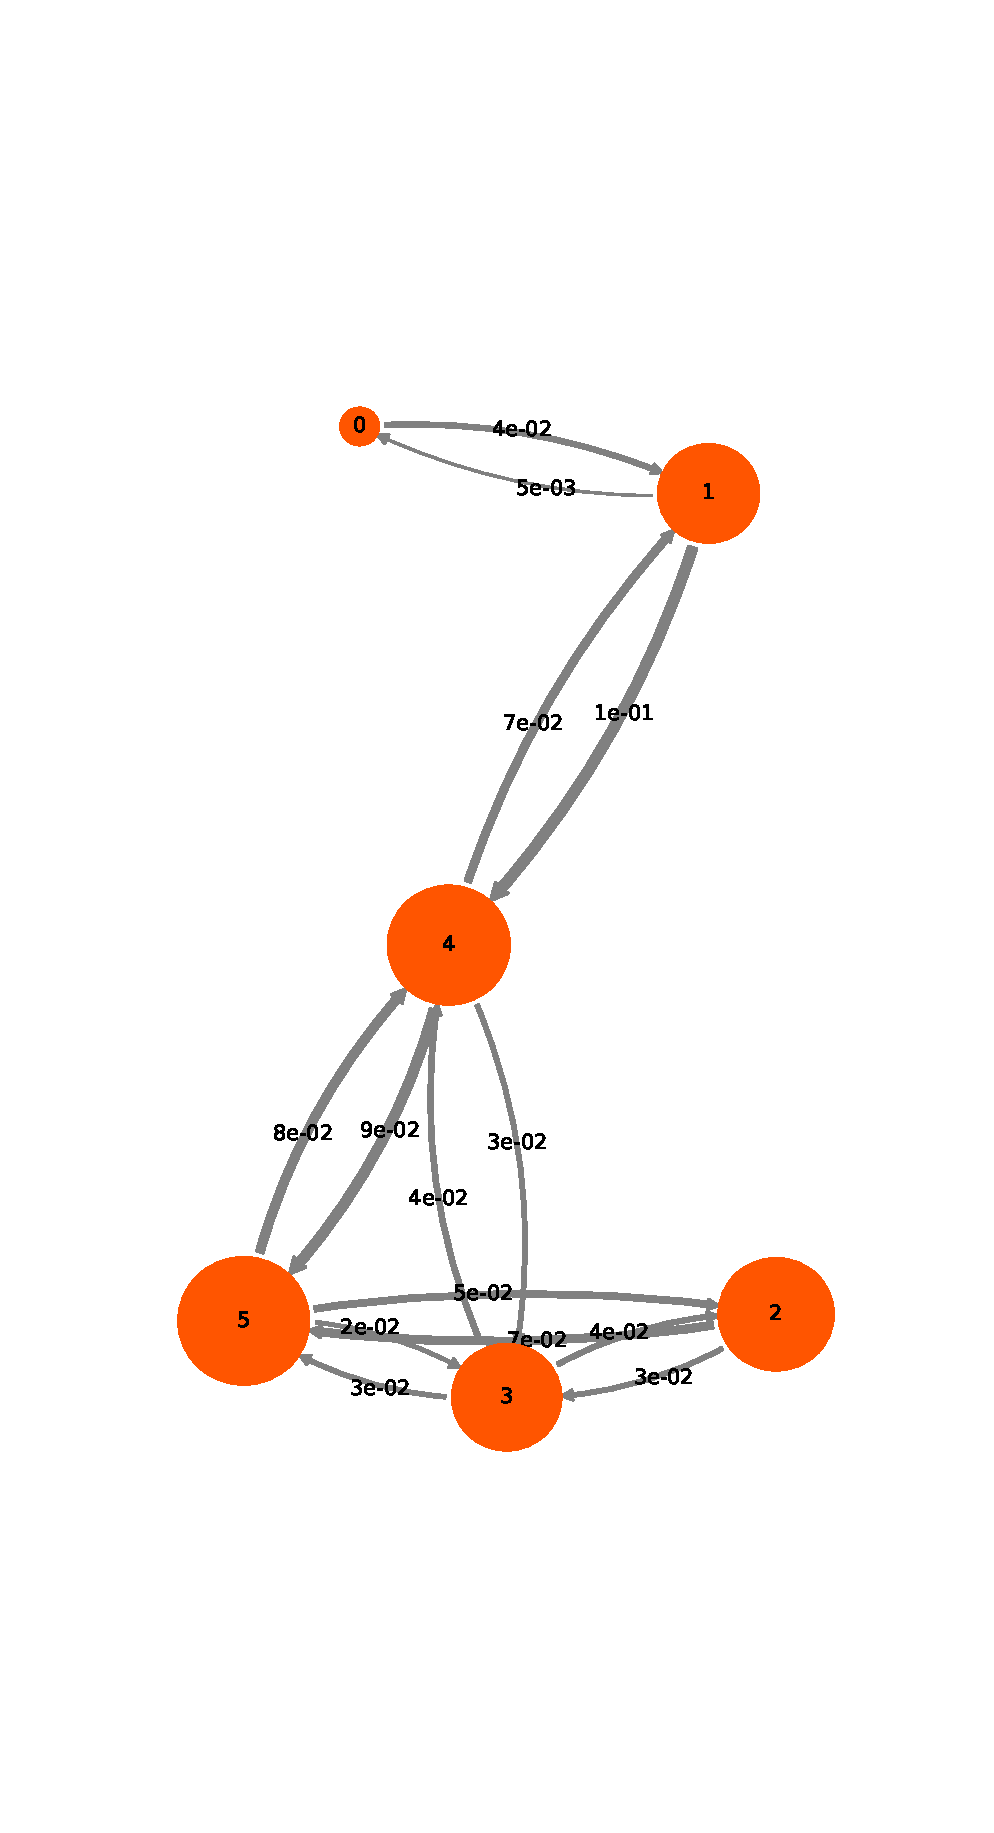
\includegraphics[width=0.65\textwidth]{./figs/fig3-05}
        \caption{The kinetic map of \ce{NaCl + 495H2O} system using a 6-state Hidden Markov Model highlighting the transition probability between 
                 each state. The average position of each index point is listed in table \ref{tab:metastable-state-indices}}
        \label{fig:hmm-6states-kineticsmodel}
    \end{figure}

    \begin{table}[h]
        \centering
        \caption{Average collective variable values for each metastable state predicted by 6-state Hidden Markov Model in figure \ref{fig:hmm-6states-kineticsmodel}}
        \label{tab:metastable-state-indices}
        \begin{tabular}{|c|c|c|c|c|}
            \hline
            \textbf{HMM State Index} & $r_{+-}$ (\r{A}) & $n_B$ & $n_+^{(1)}$ & $\rho_{ii}$ ($\mathrm{nm}^{-3}$, $\sigma = r_{+-}/4$) \\ \hline
            0 & 2.85 & 1.89 & 4.61 & 4.86 \\
            1 & 6.24 & 0.52 & 5.83 & 29.59 \\
            2 & 15.80 & 0.00 & 5.83 & 29.68 \\
            3 & 13.31 & 0.00 & 5.83 & 31.10 \\
            4 & 9.42 & 0.00 & 5.84 & 30.35 \\
            5 & 12.29 & 0.00 & 5.83 & 29.92 \\ \hline
        \end{tabular}
    \end{table}

    The indication of the CIP, SSIP, and bulk states are often judged by looking at the features of the one--dimensional free energy surface of 
    the $r_{+-}$ variable [CITE], which we have computed in chapter 5. According to the results in chapter 5, the leftmost free energy minima in 
    figure XX represents the CIP configuration, which occurs where $r_{+-} \approx 2.7$ \r{A}, while the SSIP state occurs at the second minima 
    pass the main CIP -- SSIP barrier (3.7 \r{A}) at 5.2 \r{A}. Anything beyond the second minima could be taken to be the bulk region where the 
    ions do not associate. Our results from table \ref{tab:metastable-state-indices} and figure \ref{fig:hmm-6states-kineticsmodel} indicate that 
    the dynamics spend far greater time in the bulk region, which is represented by 4 out of 6 states in figure \ref{fig:hmm-6states-kineticsmodel}. 
    Moreover, the transition probability is also biased towards the bulk from the CIP and the SSIP state, indicating that the stationary density is 
    heavily biased towards the bulk. The SSIP state, represented by a circle number 1 in figure \ref{fig:hmm-6states-kineticsmodel}, only connects 
    to one bulk state and does not have any connections to three other bulk states at all, indicating that the SSIP - bulk transition mostly occurs 
    from the leftmost boundary of the bulk state around 9 \r{A} separation of \ce{Na^+} and \ce{Cl^-} ions, and any other transitions between the 
    SSIP state to the bulk regions with higher $r_{+-}$ than 9 \r{A} is not likely to happen. A small CIP state dot of figure 
    \ref{fig:hmm-6states-kineticsmodel} implies that the dynamics spends far less time in the CIP region than other regions, with the interstate 
    transition probability biased towards the SSIP state from the CIP state.

    The information from the 6-state HMM can also be interpreted in terms of the average value of the important collective variables to elucidate 
    important information on how each configuration is arranged in the collective variable space. In terms of the coordination number of the cation, 
    it is interesting to note that the average cation coordination number for the CIP state is 4.61, which indicates that the CIP structure of NaCl 
    can either have the 4-fold coordination or the 5-fold coordination, with a slight tendency toward a 5-fold coordination, while for both SSIP 
    and bulk states, the average cation coordination number remains stable at 5.8, suggesting that both the SSIP and the bulk states prefer a 6-fold 
    coordination number, with slight possibility of the formation of a 5-fold coordinated complex. In terms of the water density around the midpoint 
    between the ions, $\rho_{ii}$ value of the CIP state is very low, because as the two ions are contacted, there is simply not enough space for 
    the water molecules to distribute around such a point in a very small volume $V_{ii} = (2\pi\sigma^2)^{3/2}$ except the water molecules of the 
    first salvation shells of the ions. As the ions become more separated, $V_{ii}$ becomes larger, allowing more water molecules to be distributed 
    around a point, and we could see that $\rho_{ii}$ values are about the same for both the SSIP and the CIP states. Another feature that 
    distinguishes the CIP, SSIP, and the bulk state is $n_B$, where the average value of $n_B$ is 1.89 for the CIP metastable states, indicating 
    that there are likely to be 2 water molecules simultaneously coordinating both the ions at the same time, which is possible due to the close 
    contact between the ions. For the SSIP, the number is likely to be 1 due to the further separation between the two ions, where a water molecule 
    between the two ions need to exist in a bridge formation spanning the entire length profile of the water molecules to accommodate both ions at 
    a distance around 5 to 6 \r{A}. For the bulk states, the number of $n_B$ is consistently zero due to the fact that the ions are now further apart, 
    so no water molecules can be simultaneously coordinating with both the ions at the same time.

    Although the results from figure \ref{fig:hmm-6states-kineticsmodel} and table \ref{tab:metastable-state-indices} gave a good idea of the 
    relative probability between each metastable states as well as how they are arranged in the collective variable space, it does not give a good 
    idea about the mechanistic point of view for this process. In order to do this, we need free energy surfaces to assist the interpretation of 
    the metastable states generated with HMM. According to figure XX, the metastable states in figure \ref{fig:hmm-6states-kineticsmodel} still 
    lacks the information from the region where $r_{+-} \approx 5.0$ \r{A}, which is a region where we expect the SSIP state for this potential. 
    Hence, we increased the metastable state approximation by HMM from 6 to 20 states to observe a better metastable state assignment. With the 
    new 20-state HMM metastable states, we could project these points obtained from HMM onto any spaces we wish and superimpose them with the free 
    energy landscapes. Figure \ref{fig:free-energy-20states-hmm-tics} represents the projection of those 20 metastable states from HMM onto the 
    space of $\tilde{\psi}_2$ and $\tilde{\psi}_3$.

    \begin{figure}[H]
        \centering
        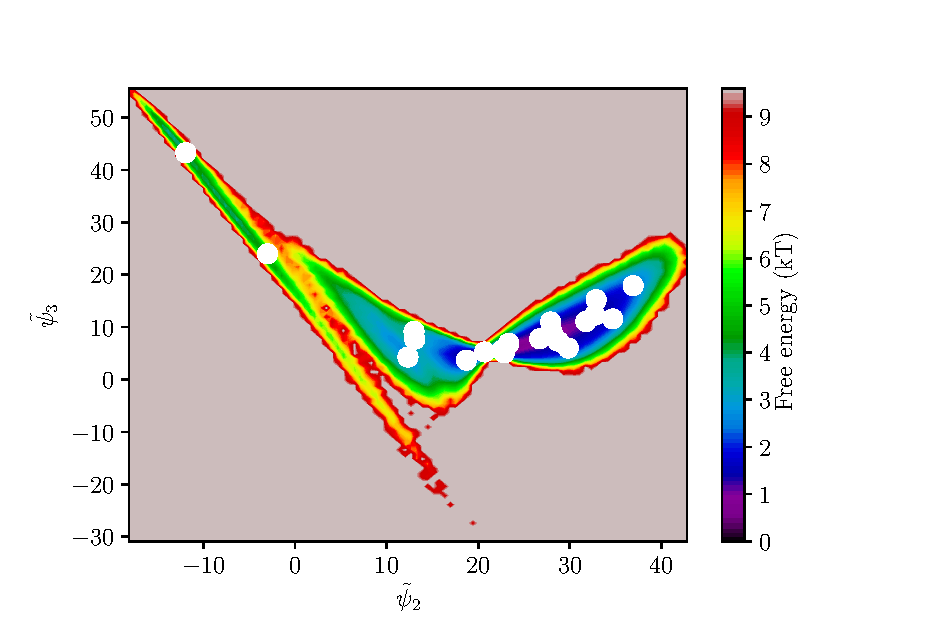
\includegraphics[width=0.85\textwidth]{./figs/fig3-06}
        \caption{Two-dimensional free energy landscape projection onto the space of $\tilde{\psi}_2$ and $\tilde{\psi}_3$, with the 20 metastable 
                 states from HMM superimposed as white dots}
        \label{fig:free-energy-20states-hmm-tics}
    \end{figure}

    The projection in figure \ref{fig:free-energy-20states-hmm-tics} was done with two of the slowest reaction coordinates obtained earlier in 
    section \ref{ssec:tica-results} using TICA, where the relative free energy is computed directly from the probability of a particular 
    configuration with respect to all configurations in the space of $\tilde{\psi}_2$ and $\tilde{\psi}_3$ according to the following equation,

    \begin{equation}
        A_i(\tilde{\psi}_2,\tilde{\psi}_3) = -\beta^{-1}\ln p_i(\tilde{\psi}_2,\tilde{\psi}_3)
    \end{equation}

    \noindent where $p_i(\tilde{\psi}_2,\tilde{\psi}_3)$ is calculated from the histogram of the bins in the $\tilde{\psi}_2$ and $\tilde{\psi}_3$ 
    space, and $\beta^{-1} = k_B T$. The free energy projection in this space shows three distinct minima; one large minimum to the right, one 
    small purple minimum to the middle, and one narrow green minimum to the left. The arrangement of these 3 main minima supports the view of the 
    ionic association as being classified into CIP, SSIP, and the bulk, where the large blue minimum corresponds to the bulk, the small purple 
    minimum corresponds to the SSIP structure, and the narrow green minimum to the left corresponds to the CIP region. However, the mechanistic 
    interpretation of this process would rely on how well do we understand how each reaction coordinate changes from the bulk states to the SSIP, 
    and eventually, to the CIP state. In order to make such interpretations, two more free energy projections are performed --- the projection onto 
    the $r_{+-}$ and the $n_B$ space to describe the behavior of $\tilde{\psi}_2$, and the projection onto the $r_{+-}$ and the $\rho_{ii}$ (feature 
    10, $\sigma = r_{+-}/3$) space to describe the behavior of $\tilde{\psi}_3$, as $n_B$ and $\rho_{ii}$ are the collective variables that correlate 
    well with $\tilde{\psi}_2$ and $\tilde{\psi}_3$, respectively. Both of these free energy projections are illustrated in figures 
    \ref{fig:free-energy-psi2} and \ref{fig:free-energy-psi3}.

    \begin{figure}[H]
        \centering
        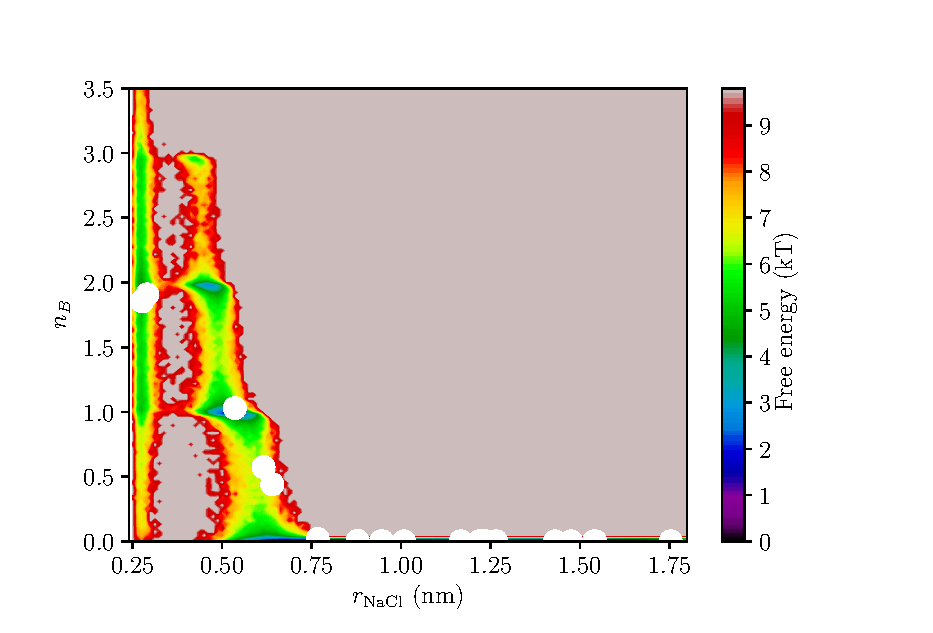
\includegraphics[width=0.85\textwidth]{./figs/fig3-07}
        \caption{Two-dimensional free energy landscape projection onto the two collective variables’ space: $r_{+-}$ and $n_B$, with the 20 metastable 
                 states from HMM superimposed as white dots}
        \label{fig:free-energy-psi2}
    \end{figure}

    \begin{figure}[H]
        \centering
        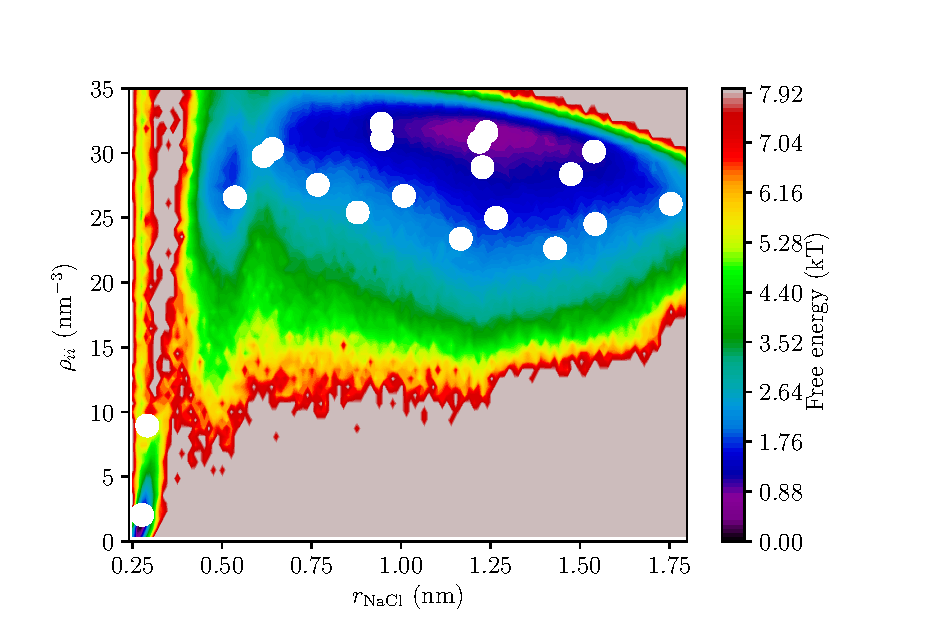
\includegraphics[width=0.85\textwidth]{./figs/fig3-08}
        \caption{Two-dimensional free energy landscape projection onto the two collective variables’ space: $r_{+-}$ and $\rho_{ii}$ (feature 10, 
                 $\sigma = r_{+-}/3$), with the 20 metastable states from HMM superimposed as white dots}
        \label{fig:free-energy-psi3}
    \end{figure}

    The free energy projection in the $r_{+-}$ and the $n_B$ space allows us to interpret the mechanistic picture of $\tilde{\psi}_2$, which is a 
    coordinate that is influenced mostly by these two collective variables. Figure \ref{fig:free-energy-psi2} implies that the transition from bulk 
    into the CIP state in the $\tilde{\psi}_2$ coordinate involves the association of the ion, with one water molecule associating both of the ion 
    in the SSIP state. The SSIP - CIP transition, according to figure \ref{fig:free-energy-psi2}, is likely driven by the water molecule in the 
    first salvation shell of either the cation and the anion associating with both the ions first to form the second bridge, and then the ions come 
    into a close contact. Nevertheless, this should not be the only possible pathway for this process, as another possible pathway from the SSIP to 
    the CIP state can also undergo the association of the ions first before the water molecules forming a bridge. Thus, the process that governs 
    the reaction coordinate $\tilde{\psi}_2$ is the driving force from the solvent bridge formation between the ions. For the reaction coordinate 
    $\tilde{\psi}_3$; however, the SSIP - CIP transition is mostly driven by the expulsion of water molecules from the region between the ions to 
    reduce the water density. As the two ions come into a close contact, the large size of the ions compared to water molecules would prohibit water 
    molecules to stay between these ions, and the nature of $\tilde{\psi}_3$ affects far more solvent molecules than the coordinate $\tilde{\psi}_2$, 
    which exerts local effect.
\end{spacing}
